% Created by tikzDevice version 0.10.1 on 2016-04-19 09:54:30
% !TEX encoding = UTF-8 Unicode
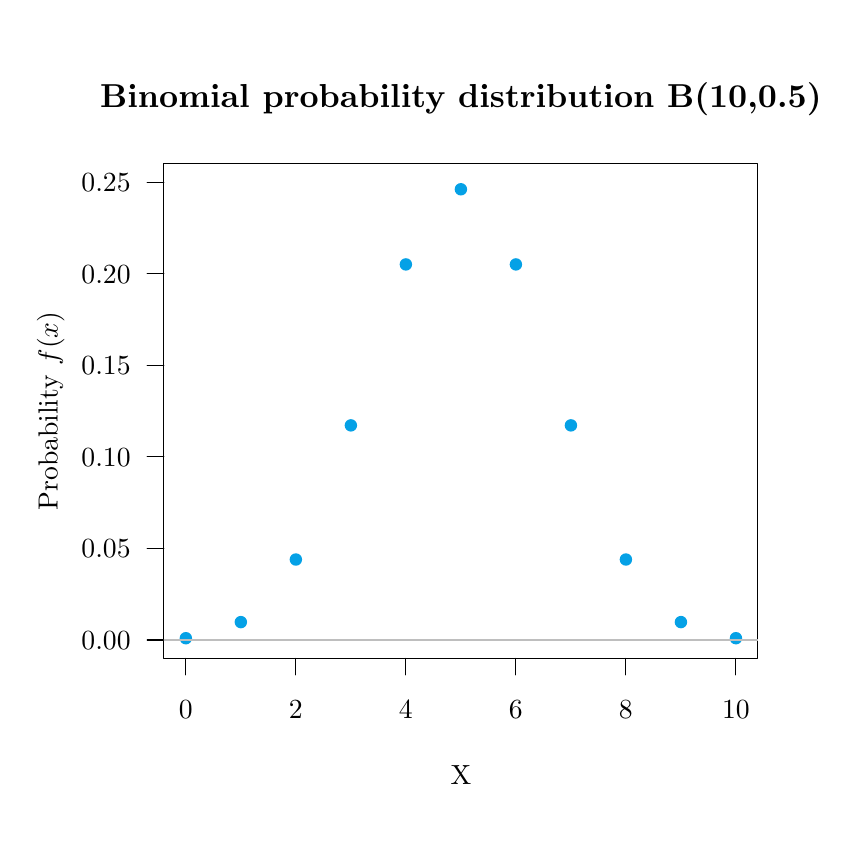
\begin{tikzpicture}[x=1pt,y=1pt]
\definecolor{fillColor}{RGB}{255,255,255}
\path[use as bounding box,fill=fillColor,fill opacity=0.00] (0,0) rectangle (289.08,289.08);
\begin{scope}
\path[clip] ( 49.20, 61.20) rectangle (263.88,239.88);
\definecolor{fillColor}{RGB}{5,161,230}

\path[fill=fillColor] ( 57.15, 68.46) circle (  2.25);

\path[fill=fillColor] ( 77.03, 74.28) circle (  2.25);

\path[fill=fillColor] ( 96.91, 96.90) circle (  2.25);

\path[fill=fillColor] (116.78,145.37) circle (  2.25);

\path[fill=fillColor] (136.66,203.53) circle (  2.25);

\path[fill=fillColor] (156.54,230.68) circle (  2.25);

\path[fill=fillColor] (176.42,203.53) circle (  2.25);

\path[fill=fillColor] (196.30,145.37) circle (  2.25);

\path[fill=fillColor] (216.17, 96.90) circle (  2.25);

\path[fill=fillColor] (236.05, 74.28) circle (  2.25);

\path[fill=fillColor] (255.93, 68.46) circle (  2.25);
\end{scope}
\begin{scope}
\path[clip] (  0.00,  0.00) rectangle (289.08,289.08);
\definecolor{drawColor}{RGB}{0,0,0}

\path[draw=drawColor,line width= 0.4pt,line join=round,line cap=round] ( 57.15, 61.20) -- (255.93, 61.20);

\path[draw=drawColor,line width= 0.4pt,line join=round,line cap=round] ( 57.15, 61.20) -- ( 57.15, 55.20);

\path[draw=drawColor,line width= 0.4pt,line join=round,line cap=round] ( 96.91, 61.20) -- ( 96.91, 55.20);

\path[draw=drawColor,line width= 0.4pt,line join=round,line cap=round] (136.66, 61.20) -- (136.66, 55.20);

\path[draw=drawColor,line width= 0.4pt,line join=round,line cap=round] (176.42, 61.20) -- (176.42, 55.20);

\path[draw=drawColor,line width= 0.4pt,line join=round,line cap=round] (216.17, 61.20) -- (216.17, 55.20);

\path[draw=drawColor,line width= 0.4pt,line join=round,line cap=round] (255.93, 61.20) -- (255.93, 55.20);

\node[text=drawColor,anchor=base,inner sep=0pt, outer sep=0pt, scale=  1.00] at ( 57.15, 39.60) {0};

\node[text=drawColor,anchor=base,inner sep=0pt, outer sep=0pt, scale=  1.00] at ( 96.91, 39.60) {2};

\node[text=drawColor,anchor=base,inner sep=0pt, outer sep=0pt, scale=  1.00] at (136.66, 39.60) {4};

\node[text=drawColor,anchor=base,inner sep=0pt, outer sep=0pt, scale=  1.00] at (176.42, 39.60) {6};

\node[text=drawColor,anchor=base,inner sep=0pt, outer sep=0pt, scale=  1.00] at (216.17, 39.60) {8};

\node[text=drawColor,anchor=base,inner sep=0pt, outer sep=0pt, scale=  1.00] at (255.93, 39.60) {10};

\path[draw=drawColor,line width= 0.4pt,line join=round,line cap=round] ( 49.20, 67.82) -- ( 49.20,233.26);

\path[draw=drawColor,line width= 0.4pt,line join=round,line cap=round] ( 49.20, 67.82) -- ( 43.20, 67.82);

\path[draw=drawColor,line width= 0.4pt,line join=round,line cap=round] ( 49.20,100.91) -- ( 43.20,100.91);

\path[draw=drawColor,line width= 0.4pt,line join=round,line cap=round] ( 49.20,134.00) -- ( 43.20,134.00);

\path[draw=drawColor,line width= 0.4pt,line join=round,line cap=round] ( 49.20,167.08) -- ( 43.20,167.08);

\path[draw=drawColor,line width= 0.4pt,line join=round,line cap=round] ( 49.20,200.17) -- ( 43.20,200.17);

\path[draw=drawColor,line width= 0.4pt,line join=round,line cap=round] ( 49.20,233.26) -- ( 43.20,233.26);

\node[text=drawColor,anchor=base east,inner sep=0pt, outer sep=0pt, scale=  1.00] at ( 37.20, 64.37) {0.00};

\node[text=drawColor,anchor=base east,inner sep=0pt, outer sep=0pt, scale=  1.00] at ( 37.20, 97.46) {0.05};

\node[text=drawColor,anchor=base east,inner sep=0pt, outer sep=0pt, scale=  1.00] at ( 37.20,130.55) {0.10};

\node[text=drawColor,anchor=base east,inner sep=0pt, outer sep=0pt, scale=  1.00] at ( 37.20,163.64) {0.15};

\node[text=drawColor,anchor=base east,inner sep=0pt, outer sep=0pt, scale=  1.00] at ( 37.20,196.73) {0.20};

\node[text=drawColor,anchor=base east,inner sep=0pt, outer sep=0pt, scale=  1.00] at ( 37.20,229.82) {0.25};

\path[draw=drawColor,line width= 0.4pt,line join=round,line cap=round] ( 49.20, 61.20) --
	(263.88, 61.20) --
	(263.88,239.88) --
	( 49.20,239.88) --
	( 49.20, 61.20);
\end{scope}
\begin{scope}
\path[clip] (  0.00,  0.00) rectangle (289.08,289.08);
\definecolor{drawColor}{RGB}{0,0,0}

\node[text=drawColor,anchor=base,inner sep=0pt, outer sep=0pt, scale=  1.20] at (156.54,260.29) {\bfseries Binomial probability distribution B(10,0.5)};

\node[text=drawColor,anchor=base,inner sep=0pt, outer sep=0pt, scale=  1.00] at (156.54, 15.60) {X};

\node[text=drawColor,rotate= 90.00,anchor=base,inner sep=0pt, outer sep=0pt, scale=  1.00] at ( 10.80,150.54) {Probability $f(x)$};
\end{scope}
\begin{scope}
\path[clip] ( 49.20, 61.20) rectangle (263.88,239.88);
\definecolor{drawColor}{RGB}{190,190,190}

\path[draw=drawColor,line width= 0.4pt,line join=round,line cap=round] ( 49.20, 67.82) -- (263.88, 67.82);
\end{scope}
\end{tikzpicture}
